\section{数字定时、同步与CFD}\label{sec:5-4}

能量标记说明一个脉冲沉积了多少能量，时间标记则用于判断不同探测器的信号是否属于同一次退激过程。第~5.3~节的慢成形适合估计幅度；时间提取更关心前沿、局部斜率和采样位置。吴鸿毅论文介绍的前沿甄别与恒比定时，以及 Lipschutz 等人的波形处理研究，提供了从采样点建立时间估计的具体路径~\cite{wu-hongyi-2020-general-purpose-digital-daq-thesis, doctoral-r1-g32-lipschutz-2016-pixie16-ddas-timing}。

首先要区分编码粒度、采样周期、插值误差、噪声抖动与实测时间分辨。设一个粗计数周期为 $T_{\mathrm{tick}}$，仅在其内部采用 $b$ 个有效细位作均匀分数编码时，数值步长才为：
\begin{equation}\label{eq:5-4-code-step}
\delta t_{\mathrm{code}} = \frac{T_{\mathrm{tick}}}{2^b};
\end{equation}
$b$ 无量纲，其余各量均为时间。这是教学编码关系，实际字中的状态位和模块映射另见第~5.5~节及附录~E。粗计数周期也不必等于 ADC 采样周期 $T_s$。插值可报告小于 $T_s$ 的时间间隔，但重复测量的散布仍受信号、算法与时钟影响，增加存储位数不会自动缩窄时间谱。

采样周期规定观察波形的时间网格，插值则利用相邻幅度中包含的前沿信息估计网格之间的位置；它没有新增一次独立的电压测量。插值误差描述估计相对给定参考的偏离，噪声抖动描述重复测量的随机变化，实际时间谱还可能包含探测器响应和漂移。因此，报告时间性能时应同时说明输入、估计算法、参考与宽度定义。

\subsection{恒比算子、参数约定与残余走动}\label{subsec:5-4-1}

固定阈值的前沿甄别记录信号首次越阈的时刻。在相同上升形状下，大幅度脉冲通常较早越阈，因而测得时间随幅度变化。恒比定时（constant fraction discrimination，CFD）通过延迟与比例相减寻找过零点，试图降低这种时间走动（time walk）。

沿用本任务模型，令 $F[n]$ 为快滤波输出，$n$ 为采样索引，$d$ 为正整数延迟样本数，$0<f<1$ 为无量纲分数，定义：
\begin{equation}\label{eq:5-4-cn}
C[n] = F[n-d] - f F[n].
\end{equation}
$F$ 与 $C$ 具有相同的幅度单位，实际延迟为 $d T_s$。本文模型选择脉冲到达后第一个由负至非负的过零区间。若其相邻样本满足 $C[n]<0\le C[n+1]$，且 $t_n=n T_s$，两点连线的零截距为：
\begin{equation}\label{eq:5-4-linear-zc}
\widehat{t}_{\mathrm{zc}} = t_n - \frac{C[n]}{C[n+1]-C[n]} T_s.
\end{equation}
该式给出插值估计；分母须非零，并须排除基线或噪声产生的无关穿越。吴鸿毅学位论文~\cite[第~25~页，式~(1.22)]{wu-hongyi-2020-general-purpose-digital-daq-thesis}采用 $x[n]-a x[n-k]$。Lipschutz 等人~\cite[式~(3)]{doctoral-r1-g32-lipschutz-2016-pixie16-ddas-timing}令 $n=i+D$ 后则为 $\mathrm{FF}[n]-w\mathrm{FF}[n-D]$。为比较记号，假设各式输入均为同一 $F$，并令原式的 $k=D=d$，则：
\begin{equation}\label{eq:5-4-cfd-map}
Y_a[n] = F[n] - a F[n-d], \qquad C[n] = -f Y_{1/f}[n].
\end{equation}
可见，同零点需要 $a=1/f$，Lipschutz 形式同理需要 $w=1/f$，并另乘整体因子 $-f$。原文方案不能只翻转符号、保留相同分数就与本文算子等同。本文模型采用上升穿越；其它实现的过零分支须随其波形极性、参数与选根条件分别说明~\cite{wu-hongyi-2020-general-purpose-digital-daq-thesis, doctoral-r1-g32-lipschutz-2016-pixie16-ddas-timing}。

例如 Lipschutz 分路测试的优化线性参数为 $(T_r, T_g, D, w)=(6, 2, 4, 5/8)$，优化三次参数为 $(2, 0, 4, 1/8)$。前三项是样本数，对应该实验 $4\,\mathrm{ns}$ 采样周期，$w$ 无量纲；$T_r$ 和 $T_g$ 分别控制快滤波的求和长度与间隙。这些小于 1 的 $w$ 不是本文 $f$ 的倒数，因此各方案需分别选取和校准定时点。

快滤波参数也参与定时：它们改变过零附近的曲率、斜率及噪声相关性。仅更换恒比分数、保留滤波参数，并不保证仍选中了适合原波形的定时区域。比较两种算法时，应区分算子、参数优化与插值方式各自的作用。

幅度不变性仍可在各自固定算子内成立。对同形、同到达相位的 $F[n]=A g[n]$，$A>0$，$g$ 为单位形状，有 $C[n]=A C_g[n]$，故：
\begin{equation}\label{eq:5-4-amp-inv}
\widehat{t}_{\mathrm{zc}} = t_n - \frac{A C_g[n]}{A [C_g[n+1]-C_g[n]]} T_s = t_n - \frac{C_g[n]}{C_g[n+1]-C_g[n]} T_s.
\end{equation}
这要求线性处理、无噪声且选中的过零分支不变，并不保证不同算子给出同一时间戳。真实前沿形状、基线偏移、饱和或采样相位变化会留下偏差；平均时间随能量的变化与随机展宽也须分别考察。局部小噪声近似下，若无噪声 CFD 曲线 $\bar{C}(t)$ 在过零 $t_\times$ 处斜率固定且非零，时间抖动可估为：
\begin{equation}\label{eq:5-4-timing-jitter}
\sigma_t \simeq \frac{\sigma_C}{|\bar{C}'(t_\times)|}.
\end{equation}
这里 $\sigma_C$ 是过零附近经过快滤波、延迟相减及相关性传播后的有效幅度噪声标准差，不能直接以原始 ADC 样本噪声替代。实际走动的方向和能量依赖应由标定确定；CFD 也不是唯一途径，前沿插值或波形函数拟合可按信号条件选用。

\subsection{采样相位与插值的条件比较}\label{subsec:5-4-2}

事件到达时刻 $t_0$ 相对本地采样网格的相位可写为 $\phi = t_0 \bmod T_s$，其中 $0 \le \phi < T_s$。过零附近曲线若有曲率，连接两个样本的直线通常不经过连续曲线的真实零点，误差便随 $\phi$ 变化。吴鸿毅学位论文~\cite[第~92--96~页]{wu-hongyi-2020-general-purpose-digital-daq-thesis}的模拟与分路测试显示了这种相位依赖；其中关于上升沿与采样周期的经验比较属于所用信号和算法，不能推广为统一分界。

表~\ref{tab:5-4-sampling-convergence} 沿用本任务的无噪声教学模型。输入波形在 $t \ge t_0$ 时取为：
\begin{equation}\label{eq:5-4-input-pulse}
v(t) = A \left[1 - e^{-(t-t_0)/\tau_r}\right] e^{-(t-t_0)/\tau_d},
\end{equation}
此前为零；$A = 1000$ 为任意幅度单位，$\tau_r = 100\,\mathrm{ns}$，$\tau_d = 50\,\mu\mathrm{s}$，$t_0 = 500\,\mathrm{ns} + \phi$。快滤波取两个长度为 $L$、间隔为 $G$ 的矩形求和之差再除以 $L$，其中 $L T_s = 100\,\mathrm{ns}$、$G T_s = 50\,\mathrm{ns}$；CFD 采用 $d T_s = 80\,\mathrm{ns}$ 和 $f = 0.4$，随后按前述上升过零规则插值，不作峰值取幅。

每个 $T_s$ 分别把其自身的有限延迟求和算子延拓到连续时间，再数值求该算子的上升过零根，得到参考延迟 $t_{\mathrm{ref}}$。比较的是 $\widehat{t}_{\mathrm{zc}} - (t_0 + t_{\mathrm{ref}})$。每行只扫描 $\phi/T_s = 0, 0.05, \dots, 0.95$ 这 20 个相位点；表值由既有 CSV 逐行读取，输入、程序和文件哈希见本节证据台账及附录~F。

\begin{table}[!htbp]
\centering
\caption{不同采样周期 $T_s$ 下 CFD 线性过零插值的采样相位误差收敛性对比（数据源自规范教学模型与 \texttt{sampling\_convergence.csv}，输入取 $A=1000$ 任意单位、$\tau_r = 100\text{ ns}$、$\tau_d = 50\ \mu\text{s}$、到达时刻 $t_0 = 500\text{ ns} + \phi$；快滤波参数取 $L T_s = 100\text{ ns}$、$G T_s = 50\text{ ns}$，CFD 延迟 $d T_s = 80\text{ ns}$、$f = 0.4$。参考延迟 $t_{\text{ref}}$ 由各采样周期下有限抽头算子延拓至连续时间的真实过零根确定。表中最大绝对误差仅覆盖离散采样的 20 个等间距相位点 $\phi/T_s \in \{0, 0.05, \dots, 0.95\}$，非连续全相位区间的解析全局上界；且计算在理想无噪声条件下进行，不包含真实探测器上升沿起伏、前放热噪声及电子学时钟抖动）。}
\label{tab:5-4-sampling-convergence}
\begin{tabular}{cccc}
\toprule
采样周期 $T_s$ & 采样率 & 参考延迟 $t_{\text{ref}}$ & 最大绝对误差 \\
(ns) & (MSPS) & (ns) & (ns，所采 20 相位点) \\
\midrule
10   & 100 & 157.1223 & 0.2566 \\
5    & 200 & 159.6536 & 0.1297 \\
2.5  & 400 & 160.8446 & 0.0137 \\
1.25 & 800 & 161.4716 & 0.0060 \\
\bottomrule
\end{tabular}
\end{table}

\begin{figure}[!htbp]
\centering
\IfFileExists{Img/cfd-phase-convergence.pdf}{%
  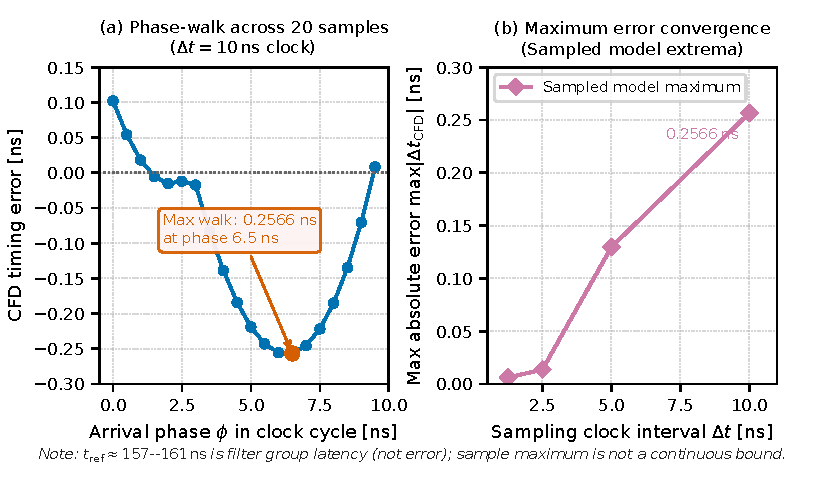
\includegraphics[width=0.85\textwidth]{Img/cfd-phase-convergence.pdf}%
}{%
  \fbox{\parbox{0.85\textwidth}{\centering\vspace{2cm}（图 5.2 待 G80 注入：\texttt{Img/cfd-phase-convergence.pdf}；展示不同采样周期下 CFD 过零插值误差随到达相位 $\phi/T_s$ 的演化曲线）\vspace{2cm}}}%
}
\caption{数字 CFD 过零插值误差随采样相位变化的收敛特征（教学模型，基于附录~F 与 \texttt{sampling\_convergence.csv}，展示采样周期在 $10\text{ ns}$、$5\text{ ns}$、$2.5\text{ ns}$ 与 $1.25\text{ ns}$ 下，20 个离散相位点上的插值时间误差。该结果说明了减小采样周期对过零曲率插值偏差的压制规律；须注意这属于理想无噪声波形在离散网格上的纯算法特征，实际系统时间分辨由信号前沿起伏、噪声抖动与时钟质量共同主导）。}
\label{fig:5-4-cfd-phase-convergence}
\end{figure}

表~\ref{tab:5-4-sampling-convergence} 中的最大值只针对所采点集，不是连续相位全区间的严格上界。减小 $T_s$ 时，各行的有限抽头结构及其连续延拓也改变，因此 $t_{\mathrm{ref}}$ 不同不代表测到了硬件走动。固定相位的幅度扫描在 $100$–$1050$ 任意单位范围内给出数值为零的时间戳散布，但仍有插值偏差；它检验同形缩放性质，不是实测零时间分辨。

幅度扫描和相位扫描回答的问题不同。前者固定采样位置，检查改变幅度是否改变结果；后者移动波形，检查同一算法是否依赖到达位置。因此，幅度缩放下完全重合的时间戳仍可共同偏离参考，不能由零散布推断估计无偏。

Lipschutz 等人~\cite{doctoral-r1-g32-lipschutz-2016-pixie16-ddas-timing}采用过零前后各两点，令局部时间坐标为 $x_j$、CFD 值为 $y_j$，求满足 $P(x_j)=y_j$ 的三次多项式 $P(x)$，$j=1,2,3,4$。这是四点多项式插值，不是三次样条。应用时应在包围所选过零的相邻样本区间内选根；若噪声导致多根或多次穿越，还需分支判别与质量控制。其改善是该实验参数优化后的结果，不能把多项式通过四点视为获得了任意波形的精确真时刻，高阶插值也可能放大噪声或引入额外振荡。

由四点确定多项式，只约束这些节点上的函数值，节点之间的真实波形仍未知。若原有过零区间内存在多个候选根，需用既定穿越方向及波形质量条件筛选，不能转而选择区间外某个更方便的根。

该研究用同一 PMT 信号分路，并给一路增加 $2\,\mathrm{ns}$ 延迟，正好为 $4\,\mathrm{ns}$ 采样周期的一半，以检验曲率相关误差。两路相位差受延迟约束，事件相对网格的绝对相位仍可随机。分路信号保留共同的探测波形变化，噪声也可同时含共模与独立分量。因此，作者先作幅度相关走动校正后得到的分路时间差谱，不能直接替代两探测器独立产生信号时的响应。

\subsection{同步、协方差与实测分辨}\label{subsec:5-4-3}

阵列同步首先要统一时钟参考和计数起点，再标定通道延迟。线缆与电路造成的偏移可在稳定时段内近似视为常数，但仍须监测温漂；相对时钟变化或抖动会改变通道间时间差。所有通道共同的全局相位平移可能在差分中消去，却不等于各模块的相对相位已稳定，更不等于单个事件的采样相位已经固定。

Hennig 等人 2007 年的 SeGA 系统以四机箱、超过 600 通道及小于 $1\,\mathrm{ns}$ 的同步波形抖动为设计目标~\cite{doctoral-r1-g32-hennig-2007-pixie16-multi-chassis-sync}。同机箱的实际测试向三模块 33 通道输入分路脉冲，对 700 组波形计算相对参考通道的时间差，所得各分布 FWHM 小于 $300\,\mathrm{ps}$。这是相对时间宽度，不另算一项独立的触发抖动测量。跨机箱测试则以示波器在数秒内累积时钟包络，模块间最大变化约 $1.5\,\mathrm{ns}$，含探头反射和失真，是最坏情况估计，既非 FWHM 也非 RMS。论文把进一步的跨机箱同步波形测试留待后续工作；这些历史记录不能充当今日模块或用户装置的保证指标。

对两路时间测量 $t_1, t_2$，在方差存在时，时间差 $\Delta t = t_1 - t_2$ 满足：
\begin{equation}\label{eq:5-4-var-dt}
\mathrm{Var}(\Delta t) = \mathrm{Var}(t_1) + \mathrm{Var}(t_2) - 2\mathrm{Cov}(t_1, t_2).
\end{equation}
各 $\sigma$ 均为时间标准差，协方差单位为时间平方。若两路具有相等、独立的 Gaussian 响应，利用 $\mathrm{FWHM} = 2\sqrt{2\ln 2}\,\sigma$，可得两通道符合谱的半高全宽满足：
\begin{equation}\label{eq:5-4-fwhm-gauss}
\mathrm{FWHM}_{\Delta t} = \sqrt{2}\,\mathrm{FWHM}_t.
\end{equation}
同源分路信号可能有相关项；若协方差为正，实测差谱可更窄；共同温度漂移常表现为正相关。相反，若系统具有周期性反相振荡或抖动，差谱将被进一步展宽。

例如，同一参考脉冲引起的共同时间偏移可在相减时抵消，但不会因此提高各通道相对外部参考的绝对稳定性。反过来，两路不相同的漂移会展宽差谱。同步标定需说明所测是通道间相对时间差还是绝对事件时刻，并报告测量时段内的漂移边界。

Lipschutz 的另一项测量以 $^{22}\mathrm{Na}$ 源照射两根 LENDA 棒，作四 PMT 符合，每棒以两端时间的均值作为棒时间，测得棒间时间差谱 FWHM 约为 $355\,\mathrm{ps}$。这是包含闪烁体光产出、光电倍增管、双端平均及特定几何配置的整体系统分辨，不是单个采样点插值误差的直接复现。探测器时间分辨由电离产生、光收集、电子倍增涨落与读出电路共同主导，数字算法只能减少后续处理中的附加展宽，无法消除传感器本征的物理涨落。

\subsection{从时间窗接受到寿命响应}\label{subsec:5-4-4}

符合窗接收的是时间差分布的一部分。若峰位随能量或通道改变，同一个窄窗可能对弱线和不同角度组合接收不同比例的真符合事件，影响强度比及方向角关联。

改善定时的谱学价值，是在保留所需真符合比例时减少混入的无关事件。对弱支路，单纯扩大窗口可能同时增加真计数和本底；强度趋于平台也未必只说明走动已被完全消除，还可能由本底补偿所致。

为说明仪器响应与核衰变的区别，可取单个能级被瞬时布居、feeding 可忽略的教学模型。假定衰变等待与仪器误差独立，且观测时段内响应稳定。令真实平均寿命为 $\tau$，仪器时间差响应为 $R(t)$，测得时间差谱为衰变指数与响应函数的时间卷积：
\begin{equation}\label{eq:5-4-st-conv}
S(t) = A_{\mathrm{sig}} \int_0^\infty \frac{e^{-u/\tau}}{\tau} R(t - t_{\mathrm{off}} - u) \, \mathrm{d}u + B(t).
\end{equation}
这里 $t$ 为测得时间差，$u$ 为真实衰变等待时间，$t_{\mathrm{off}}$ 为通道偏移；它们与 $\tau$ 使用同一时间单位。$A_{\mathrm{sig}}$ 是预期信号计数，$R$ 的单位为时间倒数，$S$ 和一般背景函数 $B$ 均为计数每单位时间，$B$ 不必平坦。此式是条件响应推导，不是三篇电子学来源中的核寿命测量。存在 feeding 时须加入相应布居时间分布，并用匹配能量、门选与通道条件的标定约束 $R$ 及其不确定度。

时间谱尾部可以同时受寿命、走动、背景和时钟变化影响；单个 FWHM 既不是寿命，也不构成寿命可辨识的硬界线，信息量还取决于统计与响应标定。具体寿命分析留待第~5.8~和~5.10~节的测量与统计语境展开。下一节转向时间标记参与触发、缓存与事件保存的过程，讨论其与联合活时间的关系。
